\documentclass[12pt, letterpaper]{article}
\usepackage[letterpaper, portrait, margin=1.25in]{geometry}
\usepackage[utf8]{inputenc}
\usepackage[english]{babel}
\usepackage{graphicx}
\usepackage{subfig}


\begin{document}

\title{%
\huge \textbf{Project Barker}\\
\large An Art Project on Social Media, Intelligent Machines, and Reality}

\author{Leo Lin, Minh Nguyen}

\maketitle

\newpage
\abstractname{ -- Project Barker is an art project that comments on the current reality of social media and human-computer interactions. Generation technology involving multiple state-of-the-art (SOTA) models helps us to build a completely "fake" Twitter. Through this interactive medium, we hope to not only trigger contemplation regarding the often underestimated power of social media and the meaning of the difference between modern social media and conventional communication technologies but also provide a space to examine humanity in front of intelligent machines and explore the boundary between the virtual world and the reality.}

\section{Introduction}

\paragraph{Social Media}Social media has become a serious societal force. It has enabled some positive change and played important roles in mass movements, such as the recent BLM movement. It also accelerates the spread of disinformation and conflict. Its potential is, so far, underestimated by the general public. Malicious entities have exploited these platforms to promote conspiracy theories, influence elections, and exacerbate genocides.

\paragraph{Artificial Intelligence}Artificial Intelligence has also profoundly impacted the world. It has transformed the medical industry, for example, with better-than-human diagnoses using computer vision and protein folding to assist drug design. However, combined with social media (in reference to recommendation algorithms), it has created echo chambers and promoted sensationalism and fake news.

\paragraph{Project Barker}Seeing that, we wanted to create a genuine yet almost satirical representation of social media and AI. Barker is a half-fledged antisocial media platform filled with AI-generated content that mimics the design of Twitter. It is not a piece of art to be marveled at, but one to experience. Exploring the app reveals information about the content’s sources and inspirations, and reading the content itself reveals not only the nature of the internet but the viewer’s very mind.

\section{Process}

\subsection{Leo Lin}

\paragraph{}My work mainly focuses on working with the various AI Models to produce the various types of images that were needed for the project. I've gathered and processed data and studied new models. I've also experimented with building my own video-generation models.

\paragraph{Image Generation}The part of my work that contributed to the final product the most is image generation. I've trained StyleGAN on multiple datasets I collected myself: emoji, Trump, Time covers, and Chinese characters. I've utilized pre-trained models such as BigGAN and AttnGAN to produce images for the final product. 

\paragraph{Data Processing}Like mentioned above, I had to collect most of the data for training the desired models. The new skills I learned includes basic web crawling and font file processing. Through the process of writing code for processing json files, transform images, filter texts, etc. I greatly improved my coding skill (in terms of data/file processing) with these experience.

\paragraph{Learning}Despite having experience with Deep Learning, I was relatively new to the realm of Natural Language Processing (NLP). So I spent many hours on teaching myself the concepts and structures SOTA NLP models (mostly Transformers). I read many papers including Transformers, BERT, ELmo, Big Bird (yes these models are actually called that, I didn't spend my SSTP watching Sesame Street), Longformer, Reformer, StyleGAN, CycleGAN, and many others to teach myself the new progresses in the field.

\paragraph{Experiments}I've also spent a lot of time attempting to construct a video-generation model based on the reformer structure with a new token mechanism. I had to abandon this plan due to the lack of time but it was a very exciting opportunity to experiment with the things I've just learned. I did not really expect this to work (my paper would be in ICCV if it actually did, video-generation is a very cutting-edge topic that still lacks satisfactory results) but the knowledge and experience I gained was totally worth the time spent.

\paragraph{Misc.}I've also gained some new experience with other rather minor things. I gained more experience with cloud computing (more time on MatPool and Google Colab, explored Kaggle, Runway ML) as most of my previous work were run on my personal node. In working with Minh, we tried to setup a remote forwarding server and an FTP server for better efficiency (an effort which Mr. Mandel also joined). I've learned how to use GitHub to manage code between multiple collaborators (all my previous use are for my own backup). I've also explored the field of video game design during the early stages of the project where we were trying to produce a film. This pursuit also sparked a conversation with Tim Oxton, a part-time photographer and video game developer. During an ealry effort of making a virtual video, I have also explored the capturing and editing of 3D scenes using a LiDAR.


\subsection{Minh Nguyen}

\section{Product Structure}

\section{Conclusion}

\paragraph{}In making the app and “creating” the content, we have improved our skills in data science, programming, and UX design. More importantly, however, we learned so much about ourselves. In reading the generated content, we explored our own thoughts and easily manipulated they are. In working on the project, we gained valuable experience with working in a team in a technical project as well as insight into what we do and do not want to do in our future careers.

\section*{Appendix}

\begin{figure}[h]
	\begin{center}
		\subfloat[\centering \linebreak]{{\includegraphics[width=0.2\linewidth]{imgs/trump/seed0233.png}}}%
    	\qquad
    	\subfloat[\centering]{{\includegraphics[width=0.2\linewidth]{imgs/trump/seed0080.png}}}%
    	\qquad
    	\subfloat[\centering]{{\includegraphics[width=0.2\linewidth]{imgs/trump/seed0292.png}}}%
    	\qquad
    	\subfloat[\centering]{{\includegraphics[width=0.2\linewidth]{imgs/trump/seed0252.png}}}%  
	\end{center}
      
    \caption{Samples Generated with StyleGAN2-ADA trained on dataset of Trump photos}
    \label{trump}
    
\end{figure}

\begin{figure}[h]
	\begin{center}
		\subfloat[\centering \linebreak]{{\includegraphics[width=0.15\linewidth]{imgs/emoji/1.png}}}%
    	\qquad
    	\subfloat[\centering]{{\includegraphics[width=0.15\linewidth]{imgs/emoji/2.png}}}%
    	\qquad
    	\subfloat[\centering]{{\includegraphics[width=0.15\linewidth]{imgs/emoji/4.png}}}%
    	\qquad
    	\subfloat[\centering]{{\includegraphics[width=0.15\linewidth]{imgs/emoji/5.png}}}%  
    	\qquad
    	\subfloat[\centering]{{\includegraphics[width=0.15\linewidth]{imgs/emoji/6.png}}}%  
	\end{center}
      
    \caption{Samples Generated with StyleGAN2-ADA trained on dataset of Trump photos}
    \label{trump}
    
\end{figure}

\begin{figure}[h!]
	\begin{center}
		\subfloat[\centering \linebreak]{{\includegraphics[width=0.25\linewidth]{imgs/time1.png}}}%
    	\qquad
    	\subfloat[\centering]{{\includegraphics[width=0.25\linewidth]{imgs/time2.png}}}%
    	\qquad
    	\subfloat[\centering]{{\includegraphics[width=0.25\linewidth]{imgs/time3.png}}}%
	\end{center}
      
    \caption{Samples Generated with StyleGAN2-ADA trained on dataset of Time magazine covers}
    \label{trump}
    
\end{figure}

\begin{figure}[h]
	\begin{center}
		\subfloat[\centering \linebreak]{{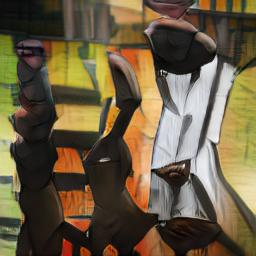
\includegraphics[width=0.25\linewidth]{imgs/attn/000001075.jpeg}}}%
    	\qquad
    	\subfloat[\centering]{{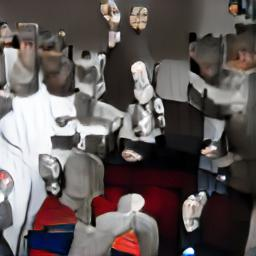
\includegraphics[width=0.25\linewidth]{imgs/attn/000000235.jpeg}}}%
    	\qquad
    	\subfloat[\centering]{{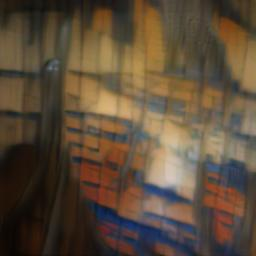
\includegraphics[width=0.25\linewidth]{imgs/attn/000000185.jpeg}}}%
    	\qquad
    	\subfloat[\centering]{{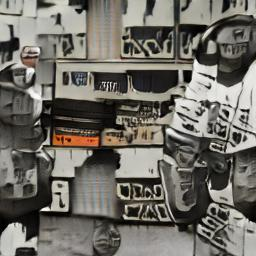
\includegraphics[width=0.25\linewidth]{imgs/attn/000000071.jpeg}}}%  
    	\qquad
    	\subfloat[\centering]{{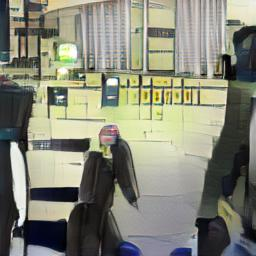
\includegraphics[width=0.25\linewidth]{imgs/attn/000000373.jpeg}}}%
    	\qquad
    	\subfloat[\centering]{{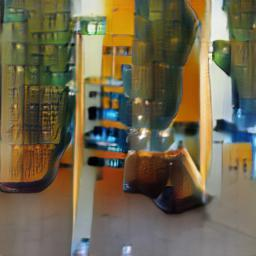
\includegraphics[width=0.25\linewidth]{imgs/attn/000000345.jpeg}}}%  
	\end{center}
      
    \caption{Samples Generated with Attention GAN with tweets}
    \label{trump}
    
\end{figure}
 
 \begin{figure}[h]
	\begin{center}
		\subfloat[\centering \linebreak church]{{\includegraphics[width=0.2\linewidth \linebreak]{imgs/big/church.jpg}}}%
    	\qquad
    	\subfloat[\centering fire truck]{{\includegraphics[width=0.2\linewidth]{imgs/big/firetruck.jpg}}}%
    	\qquad
    	\subfloat[\centering library]{{\includegraphics[width=0.2\linewidth]{imgs/big/library.jpg}}}%
    	\qquad
    	\subfloat[\centering police van]{{\includegraphics[width=0.2\linewidth]{imgs/big/policevan.jpg}}}%
    	\qquad
    	\subfloat[\centering rifle]{{\includegraphics[width=0.2\linewidth]{imgs/big/rifle.jpg}}}%
    	\qquad
    	\subfloat[\centering stage]{{\includegraphics[width=0.2\linewidth]{imgs/big/stage.jpg}}}%
    	\qquad
    	\subfloat[\centering stretcher]{{\includegraphics[width=0.2\linewidth]{imgs/big/stretcher.jpg}}}%
    	\qquad
    	\subfloat[\centering website]{{\includegraphics[width=0.2\linewidth]{imgs/big/website.jpg}}}%
    	\qquad
	\end{center}
      
    \caption{Samples Generated with Big GAN from several different categories}
    \label{trump}
    
\end{figure}

\end{document}